\section{Perché la compressione run-length}
Prima di proseguire con la spiegazione dettagliata delle varianti della
$\RLPBWT$ è bene dare 
una prima motivazione al perché si sia ritenuto utile sviluppare una variante
run-length encoded della $\PBWT$.\\
Citando direttamente il paper di Durbin \cite{pbwt}:
\begin{center}
  \textit{Furthermore we can also expect the $y$ arrays to be strongly
    run-length compressible. This is because population genetic structure means
    that there 
    is local correlation in values due to linkage disequilibrium, which means
    that haplotypes with similar prefixes in the sort order will tend to have
    the same allele values at the next position, giving rise to long runs of
    identical values in the $y$ array. So the $\PBWT$ can easily be stored in
    smaller space than the original data.} 
\end{center}
Quindi, il risultato atteso è quello per cui aplotipi simili, che, ad ogni step,
saranno consecutivi nel riordinamento inverso, è molto probabile presentino lo
stesso 
allele nella colonna di cui si sta calcolando la
permutazione. Ne segue che, all'interno della matrice $\PBWT$, è molto
probabile che si abbiano lunghe run di simboli $\sigma=0$ e di simboli
$\sigma=1$.
Si ottiene il medesimo risultato atteso avuto con
la $\BWT$, avendo che caratteri uguali è molto probabile vengano posti in
posizioni consecutive all'interno della trasformata stessa. Si hanno le
stesse premesse che hanno portato alla $\RLBWT$, considerando, inoltre,
che, non si tratta solo di memorizzare la struttura con
compressione run-length ma di lavorare direttamente con la struttura dati
compressa, risolvendo il problema del calcolo degli $\SMEM$ senza
decomprimere la struttura dati. Ipotizzando che, per una certa colonna della
matrice $\PBWT$, il numero di run sia molto minore della lunghezza della
colonna stessa, si deduce facilmente che l'uso della compressione run-length
possa comportare una riduzione significativa della memoria necessaria al calcolo
degli $\SMEM$.
\section{Matching Statistics per la RLPBWT}
Bisogna ora introdurre il 
concetto di \textbf{matching statistics} nel caso della $\PBWT$ (e quindi
anche della sua variante run-length encoded).
\begin{definizione}
  Dato un pannello $X$, di dimensioni $M\times N$, con $M$ individui e $N$ siti,
  e un aplotipo esterno/pattern $z$, tale che $|z|=N$, si definisce matching
  statistics di $z$ su $X$ un array $\MS$ di coppie $(\row,\len)$, di lunghezza
  $N$, tale che (avendo che $x_i$ indica l'$i$-esima riga del pannello $X$): 
  \begin{itemize}
    \item $x_{\MS[i].\row}[i-\MS[i].\len+1,i]=z[i-\MS[i].\len+1,i]$, ovvero si
    ha che 
    l'aplotipo query ha un match, terminante in colonna $i$, con la riga
    $\MS[i].\row$  
    \item $z[i-\MS[i].\len,i]$ non è un suffisso terminante in colonna $i$ di un
    qualsiasi sottoinsieme di righe di $X$. In altri termini, il match non deve
    essere ulteriormente estendibile a sinistra
  \end{itemize}
\end{definizione}
\noindent
Analogamente al caso della variante classica, si ha il seguente lemma.
\begin{lemma}
  Dato un pannello $X$, di dimensioni $M\times N$, con $M$ individui e $N$
  siti, un aplotipo esterno/pattern $z$, tale che $|z|=N$, e il corrispondente
  array di matching statistics $\MS$ si ha che $z[i-l+1,i]$
  presenta uno $\SMEM$ di lunghezza $l$ in con la riga $\MS[i].\row$ del pannello
  $X$ sse: 
  \begin{equation}
    \label{eq:rlpbwtsmem}
    \MS[i].\len=l\land(i=N-1\lor \MS[i].\len\geq \MS[i+1].\len)
  \end{equation}
\end{lemma}
\noindent
\textit{Si vedrà in sezione \ref{secphi} come calcolare, a partire da tali
  $\SMEM$, tutte le righe del panello per le quali si ha il medesimo
  $\SMEM$}.\\
Il calcolo dell'array $\MS$ di $z$ rispetto al pannello $X$ si basa su due fasi:
\begin{enumerate}
  \item la fase di \textbf{start}
  \item la fase di \textbf{extend}
\end{enumerate}
Si assuma di avere due indici $i$ e $j$, $0\leq i\leq j< N$, tali per cui
$z[i,j]$ è un suffisso di uno tra $x_0[0,j]$, \ldots, $x_{M-1}[0,j]$. \\
La fase di extend estende il match di $z[i,j]$ a $z[i,j+1]$ sse:
\begin{itemize}
  \item $j<M$
  \item $z[i,j+1]$ è un suffisso di uno tra $x_0[0,j+1]$, $\ldots$,
  $x_{M-1}[0,j+1]$ 
\end{itemize}
Invece, la fase di start cerca il più piccolo indice $i'$,
avendo $i\leq i'\leq j$, tale per cui $z[i',j]$ è un suffisso di uno tra
$x_0[0,j]$, $\ldots$, $x_{M-1}[0,j]$.\\
Si ha quindi il computo di ogni valore $\MS[i]$, $\forall i\in[0,N)$:
\begin{itemize}
  \item si assume inizialmente che $\MS[0].\len=0$, quando $i=0$
  \item si applica la fase di start per cercare il minimo indice
  $i'$, avendo $i\leq i'$, tale che $z[i',i'+\MS[i].\len]$ è un suffisso di uno
  tra $x_0[0,i'+\MS[i].\len], \ldots$ $x_{M-1}[0,i'+\MS[i].\len]$. Inoltre, per
  minimalità di $i'$, si ha che, $\forall i<j<i'$,
  $\MS[j].\len=\MS[j-1].\len-1$, $\forall j\in[i+1,i'-1]$
  \item si itera la fase di extend per trovare il
  più lungo prefisso $z[i',k]$ che è anche un suffisso di uno tra $x_0[0,k]$,
  $\ldots$, $x_{M-1}[0,k]$, avendo che $\MS[i'].\len=k-i'+1$
  \item avendo che $i'>i$, si può procedere induttivamente al calcolo dell'array
  $\MS$ 
\end{itemize}
Per convenzione, si ha che la riga da cui parte l'iterazione nella prima colonna
è l'ultima. Tale scelta è, in ogni caso, arbitraria.
In modo
analogo, qualora si abbia una colonna $k$ di un solo carattere, non
corrispondente a quello della query, si sceglie l'ultima riga della
colonna successiva. A partire da tale riga, si riprende il calcolo 
dell'array delle matching statistics, dopo aver memorizzato $\MS[k].\row=M$
(un valore sentinella non esistendo la riga $M$) e $\MS.\len[k]=0$.\\
In altri termini, più ``pratici'', il calcolo dell'array $\MS$ avviene nel
seguente modo:
\begin{itemize}
  \item si parte da una riga arbitraria $i$ della prima colonna
  \item se $x_i[0]=z[0]$ si procede salvando $\MS[0].\row=i$
  \item qualora si abbia $x_i[0]\neq z[0]$, si seleziona o l'ultima riga della
  run precedente o la prima riga della run successiva a quella a cui appartiene
  la riga $i$. Tale riga verrà salvata come $\MS[0].\row=j$
  \item si effettua il mapping verso la colonna successiva, $k$,
  e, a seconda di avere o meno un match con $z[k]$, si procede come nei casi
  visti sopra 
\end{itemize}
Si noti che non si è parlato di come calcolare i vari $\MS[i].\len$, in
quanto si hanno due soluzioni (approfondite in seguito), che
rispecchiano quanto visto con 
MONI \cite{moni} e PHONI \cite{phoni} per la $\RLBWT$: 
\begin{enumerate}
  \item si possono usare le threshold per capire che nuova riga
  selezionare in 
  caso di mismatch. In tal caso i valori $\MS[i].\len$ devono essere calcolati
  successivamente al calcolo dei valori $\MS[i].\row$ tramite random
    access al panel 
  \item si possono usare le $\LCE$ query per capire quale nuova riga
  selezionare in caso di mismatch. In tal caso il calcolo dei valori
  $\MS[i].\len$ avviene in contemporanea al calcolo dei valori $\MS[i].\row$
\end{enumerate}
\begin{esempio}
  \label{es:ms}
  Si riprenda, al fine di vedere un esempio di calcolo dell'array $\MS$,
  l'esempio \ref{es:algo5}, con un pannello e i match con 
  la query $z$:
  \begin{figure}[H]
    \centering
    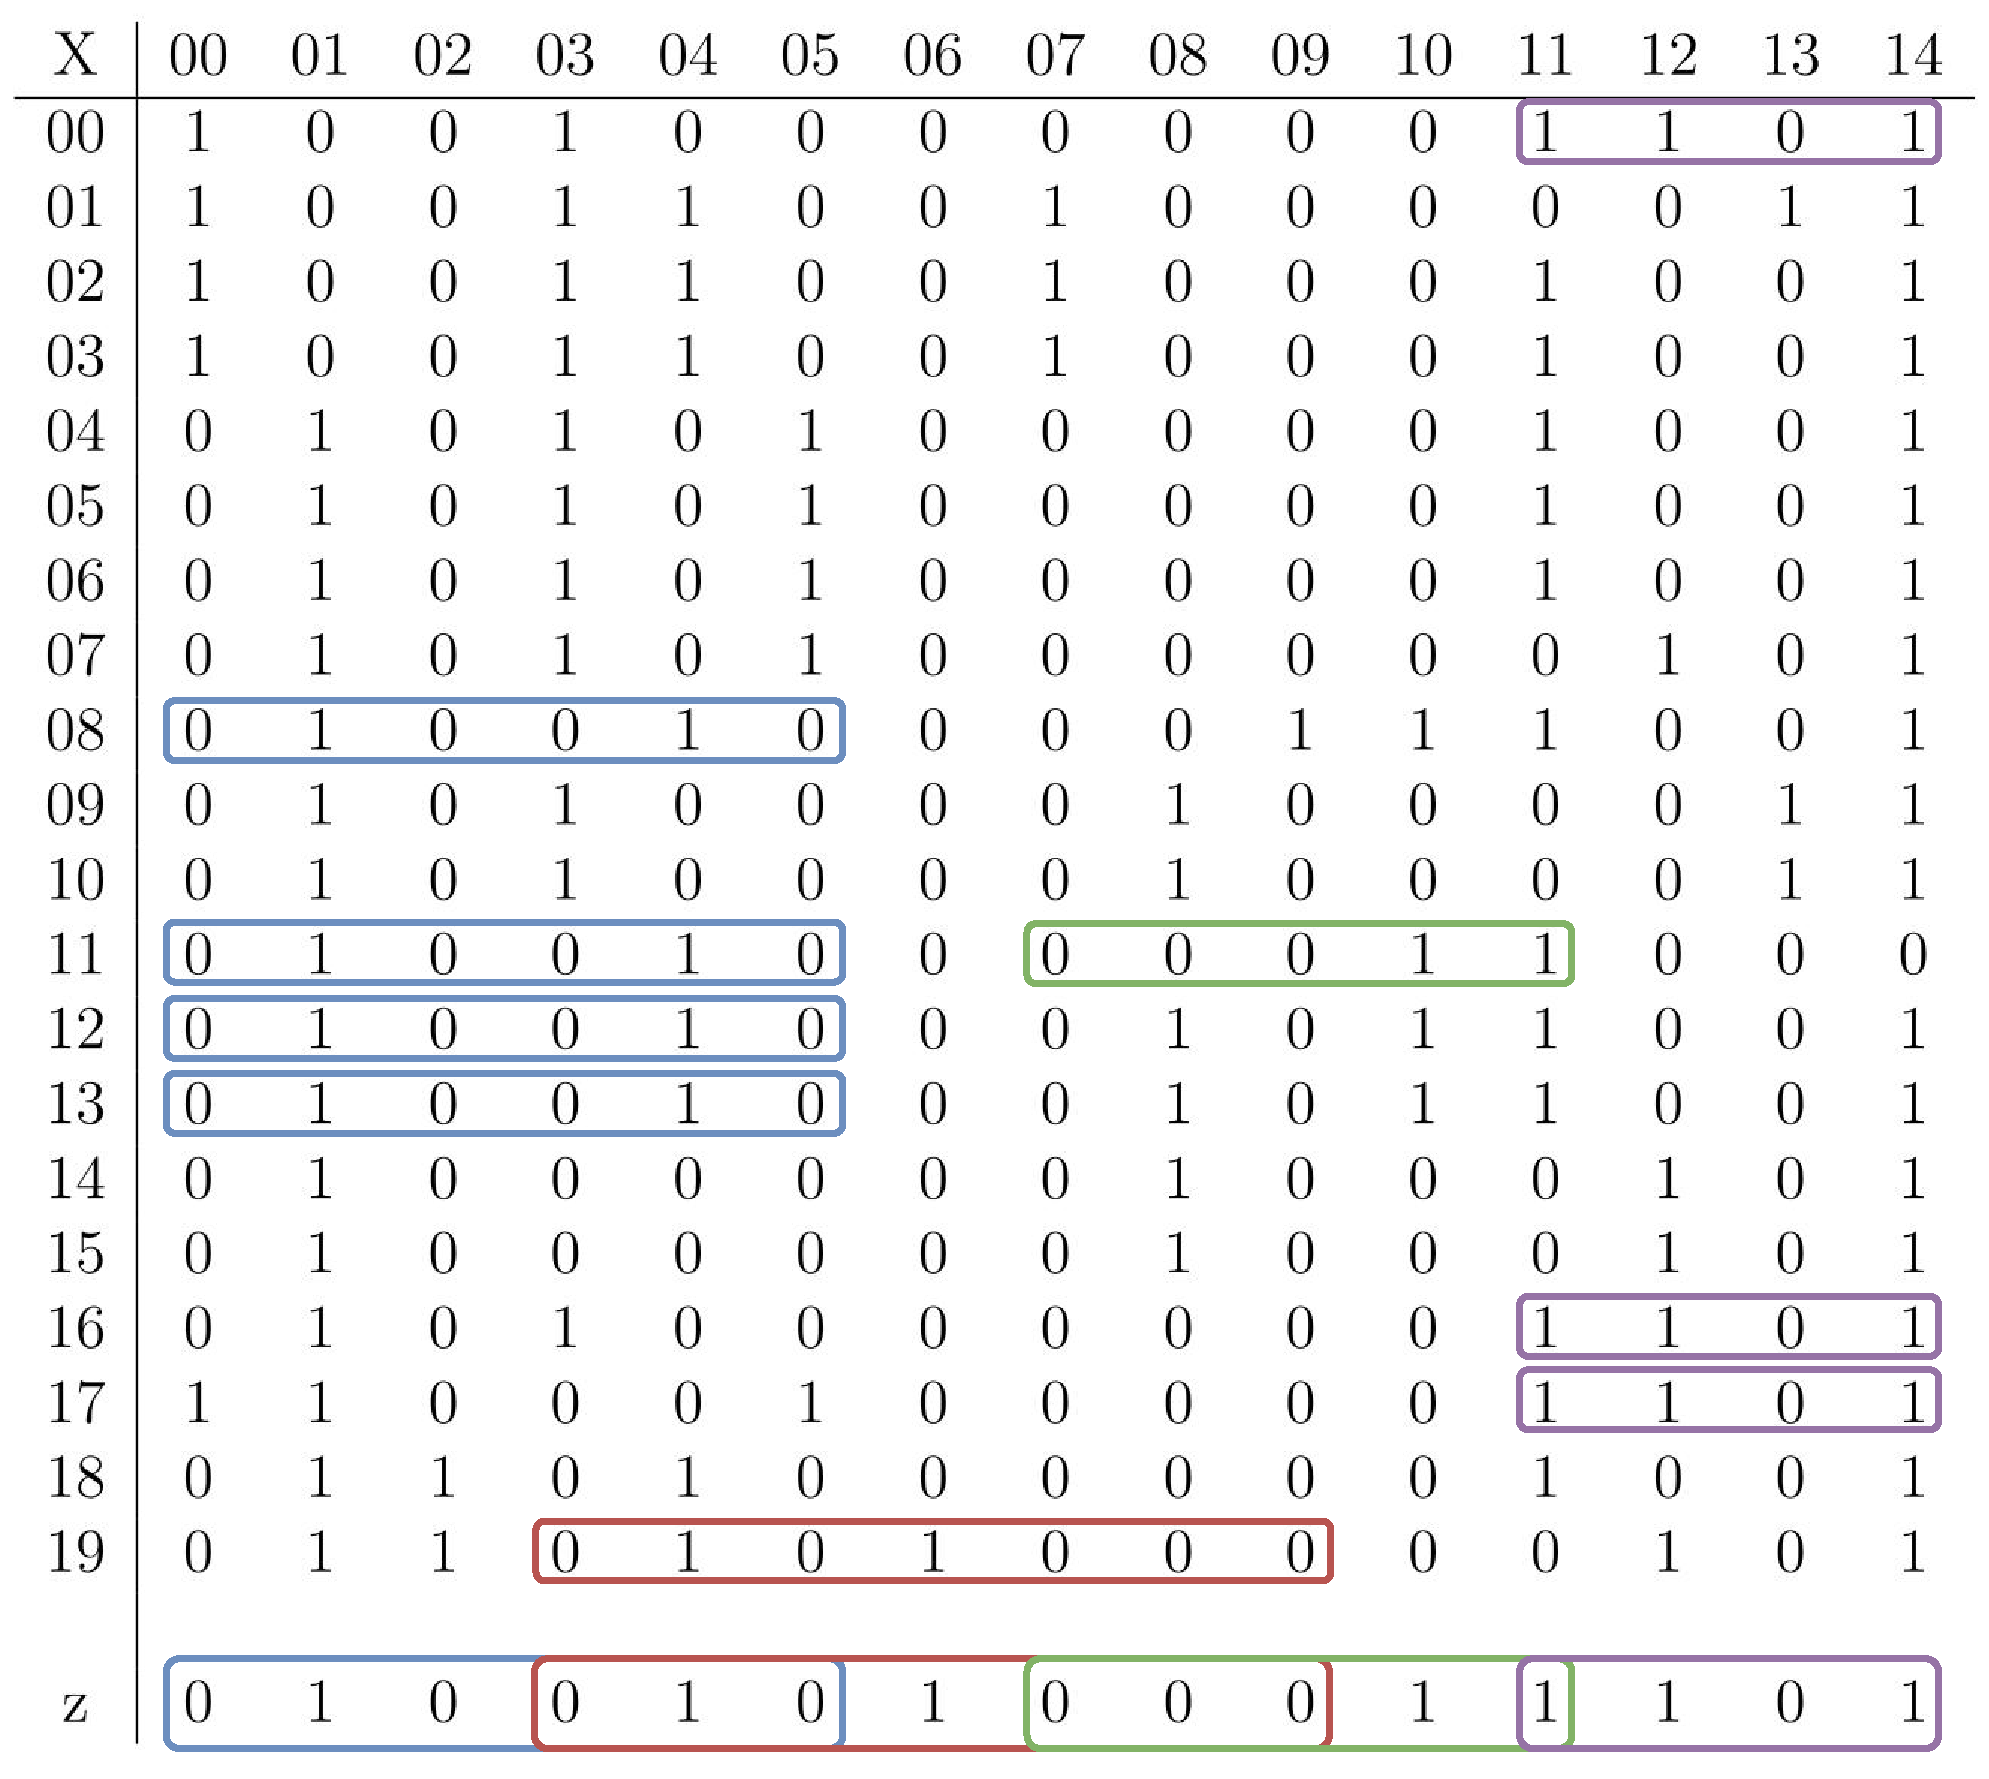
\includegraphics[scale = 0.365]{img/pbwtmatch.pdf}
  \end{figure}
  In tal caso l'array $\MS$ sarebbe, avendo scelto come riga iniziale la 19:
  \begin{table}[H]
    \footnotesize
    \centering
    \begin{tabular}{c|ccccccccccccccc}
      $k$ & 00 & 01 & 02 & 03 & 04 &  {\color{nordcyan}05} & 06 & 07 & 08
      &  {\color{nordred}09} & 10 &  {\color{nordgreen}11} & 12 & 13
      &  {\color{nordpurple}14} \\
      \hline
      \hline
      $z$ & 0 & 1 & 0 & 0 & 1 &  {\color{nordcyan}0} & 1 & 0 & 0
      &  {\color{nordred}0} & 1 &  {\color{nordgreen}1} & 1 & 0
      &  {\color{nordpurple}1} \\
      \hline
      $\row$ & 19 & 19 & 16 & 15 & 13 &  {\color{nordcyan}13} & 19 & 19 & 19
      &  {\color{nordred}19} & 11 &  {\color{nordgreen}11} & 17 & 17
      &  {\color{nordpurple}17} \\
      $\len$ & 1 & 2 & 3 & 4 & 5 & {\color{nordcyan}6} & 4 & 5 & 6
      & {\color{nordred}7} & 4 & {\color{nordgreen}5} & 2 & 3
      & {\color{nordpurple}4}\\
    \end{tabular}
  \end{table}
  Dove si possono riconoscere i vari $\SMEM$, la cui colonna di fine è
  segnalata nello stesso colore con cui si rappresentano gli $\SMEM$ nel
  pannello. Anche in questo caso i dettagli del calcolo 
  verranno esplicitati successivamente. 
\end{esempio}
\section{Componenti per la RLPBWT}
Questo progetto di tesi è stato è stato incentrato sullo sviluppo di
varie implementazioni della $\RLPBWT$. Infatti, avendo a che fare con
strutture dati fortemente dipendenti dal tipo di dato (in termini, ad esempio,
di ``sparsità'' intrinseca del pannello) e dall'implementazione (soprattutto in
termini di strutture dati succinte), sarebbe stato difficile limitarsi a stime
teoriche che potevano non essere confermate in fase sperimentale. Una sola
caratterizzazione asintotica avrebbe potuto comportare sottostime e
sovrastime, sia in termini di tempo che di spazio. Quindi, si deciso di
sviluppare diverse varianti della $\RLPBWT$.\\ 
Al fine di una miglior trattazione di tali implementazioni, si è deciso di
suddividere le stesse in componenti, le quali, adeguatamente
assemblate, permetteranno il calcolo degli
$\SMEM$. Tali componenti, che verranno dettagliate in seguito, sono:
\begin{itemize}
  \item le componenti per il mapping tra la colonna $k$-esima e la colonna
  $k+1$, ovvero, riprendendo la notazione di Durbin, le strutture run-length
  encoded per gli array $c$, $u_k$ e $v_k$. Nel dettaglio, tale componente è
  implementata in due varianti:
  \begin{enumerate}
    \item mapping tramite intvector (\texttt{MAP-INT})
    \item mapping tramite bitvector sparsi (\texttt{MAP-BV})
  \end{enumerate}
  \item la componente per la memorizzazione delle threshold, anch'essa
  proporzionale al numero di run. Anche in questo caso si hanno due varianti,
  corrispondenti, di fatto, alle due varianti della componente del mapping:
  \begin{enumerate}
    \item threshold con intvector (\texttt{THR-INT})
    \item threshold con bitvector sparsi (\texttt{THR-BV})
  \end{enumerate}
  \item la componente per la memorizzazione compatta della permutazione ad ogni
  colonna 
  della matrice $\PBWT$, ovvero dei sample di prefix array
  (\texttt{PERM}) 
  \item la componente in grado di garantire random access al
  pannello. Si hanno due possibilità:
  \begin{enumerate}
    \item random access con bitvector (\texttt{RA-BV})
    \item random access con SLP (\texttt{RA-SLP})
  \end{enumerate}
  \item la componente per le longest common extension query
  (\texttt{LCE}) 
  \item la componente per l'intero reverse longest common prefix array
  (\texttt{RLCP}), già descritto nella sezione \ref{secpbwt}
  \item la componente per permettere il calcolo delle funzioni
  $\varphi$ e $\varphi^{-1}$ (\texttt{PHI})
\end{itemize}


% Tali varianti non sono da
% intendersi ugualmente valide ma corrispondono al percorso evolutivo avuto
% nell'ultimo anno di studio e ricerca in merito. Riassumendo il tutto si
% vedranno:
% \begin{itemize}
%   \item una prima implementazione \textit{na\"{i}ve}, detta appunto
%   \textbf{RLPBWT na\"{i}ve}, che corrisponde al primo tentativo di studio. Tale
%   versione è stata 
%   fortemente ispirata dai risultati introduttivi di Gagie et
%   al. \cite{tricks}. Questa soluzione non 
%   permette di sapere quali righe del pannello presentano uno \textit{SMEM},
%   terminante in una certa colonna, ma solo quante
%   \item si è quindi iniziato ad introdurre l'uso dei \textit{bitvector sparsi},
%   con la 
%   \textbf{RLPBWT con bitvectors}, il cui funzionamento è pressoché analogo alla
%   versione \textit{na\"{i}ve}, al più dell'uso di tali strutture succinte per il
%   funzionamento del mapping. Questa soluzione non
%   permette di sapere quali righe del pannello presentano uno \textit{SMEM},
%   terminante in una certa colonna, ma solo quante
%   \item il primo sostanziale ``cambio di paradigma'', si ha avuto con la
%   \textbf{RLPBWT con pannello denso}, variante in cui, oltre all'uso dei
%   \textit{bitvectors} si è proceduto al calcolo degli \textit{SMEM} tramite
%   \textit{matching statistics} e \textit{LCE query}. Questa soluzione permette
%   di sapere l'indice di una sola riga per la quale si sta avendo uno
%   \textit{SMEM}, terminante in una certa colonna, con il pattern 
%   \item migliorando la soluzione precedente con l'uso dell'\textit{SLP} per la
%   memorizzazione del pannello si è ottenuta la \textbf{RLPBWT con SLP}. Questa
%   soluzione permette di sapere l'indice di una sola riga per la quale si sta
%   avendo uno \textit{SMEM}, terminante in una certa colonna, con il pattern 
%   \item infine, con l'implementazione delle \textbf{funzioni}
%   $\boldsymbol\varphi$ e $\boldsymbol\varphi^\mathbf{-1}$ per la 
%   \textbf{RLPBWT}, si è permesso di estendere i risultati delle ultime due
%   varianti in modo da ottenere tutti gli \textit{SMEM} con tutti gli indici
%   delle righe per cui si ha il medesimo \textit{SMEM} con il pattern
% \end{itemize}
% Si può quindi iniziare ad apprezzare il percorso evolutivo e incrementale
% vissuto con questo progetto.

% LocalWords:  sovrastime
